\ca{\chapter{User Guide}}
\renewcommand{\baselinestretch}{\mystretch}
\label{chap:Guide}
%\setlength{\parindent}{0pt}

\section{Sequence exporting}

To export sequence designs for the playback engine, open the \textit{Export Sequence} dialog from \textit{Timed Sequence Editor}, under menu \textit{Sequence} $\rightarrow$ \textit{Export}. (\fref{fig:guide_export})

\begin{figure}[!htb]
  \centering
  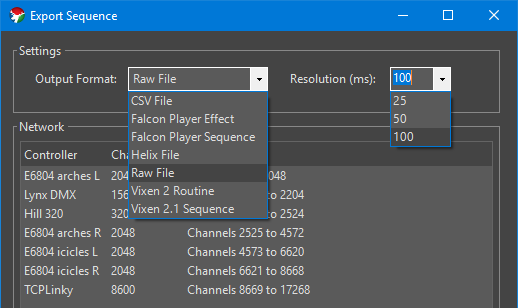
\includegraphics[width=0.75\columnwidth]{Figs/vixen_export.png}
  \caption{\footnotesize Sequence export dialog}
  \label{fig:guide_export}
\end{figure}

Select \textit{Raw File} as \textit{Output Format}, and configure the required frame interval at \textit{Resolution (ms)}. All the controller channels listed in \textit{Network} will be exported.

Click on \textit{Start}, select a sequence save location, the export process should be started. It may take a few minutes to render the sequence.

Two files will be created, the selected \texttt{*.raw} file and a network configuration file \texttt{*\_Network.xml}. The sequence file and an optional audio file will be specified in the network configuration file. In case their file names or paths changed, the relevant fields in the network configuration file should be updated as well.

\section{Video transcoding tool}

A CUI tool \texttt{codec.exe} is available for transcoding the exported \textit{Raw File} to or from a video file, \cb{independently} from the Vixen application.

\renewcommand{\baselinestretch}{1}
\begin{lstlisting}[language=]
Usage:  codec.exe input output

Supported transcoding processes:
    *_Network.xml   -> *.mp4	| Encode a raw sequence to a video file.
				| The video file will use h264 encoding
				| with rgb24 pixel format.
				|
    *.mp4/avi/mov.. -> *.raw	| Decode a video file to a raw sequence,
				| *_Network.xml will also be created.

Examples:
    codec.exe exported_Network.xml exported.mp4
    codec.exe exported.mp4 exported.raw
\end{lstlisting}
\renewcommand{\baselinestretch}{\mystretch}

\section{Invoke the playback engine from GUI}

The playback engine can be accessed from the main window, under menu \textit{Tools} $\rightarrow$ \textit{Playback}. (\fref{fig:guide_playback})

\begin{figure}[!htb]
  \centering
  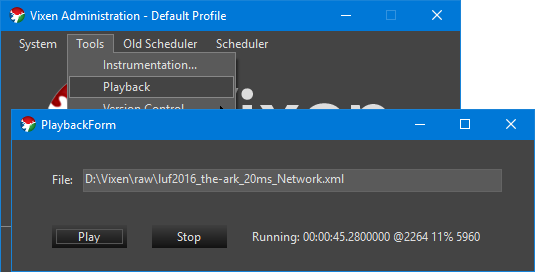
\includegraphics[width=0.7\columnwidth]{Figs/vixen_playback.png}
  \caption{\footnotesize Playback engine control dialog}
  \label{fig:guide_playback}
\end{figure}

Set a network configuration file or a video sequence file, click \textit{Play}, rendering should be started using the playback engine.

\section{Setup schedules with the playback engine}

The scheduler schedules lighting shows at specific times. To create or modify a show, open the show setup dialog from the main window, under menu \textit{Scheduler} $\rightarrow$ \textit{Shows}.

Different actions can be added to different stages of a show. The playback engine can be scheduled by adding an action of type \textit{Playback}, with a network configuration file or a video sequence file as input. (\fref{fig:guide_show})

\begin{figure}[!htb]
  \centering
  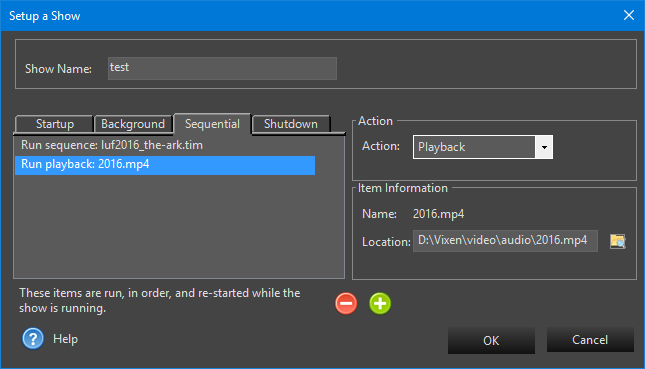
\includegraphics[width=0.8\columnwidth]{Figs/vixen_show.png}
  \caption{\footnotesize Show setup dialog}
  \label{fig:guide_show}
\end{figure}

After creating a show, the scheduler can be accessed from the main window, under menu \textit{Scheduler} $\rightarrow$ \textit{Schedules}. (\fref{fig:guide_scheduler})

\begin{figure}[!htb]
  \centering
  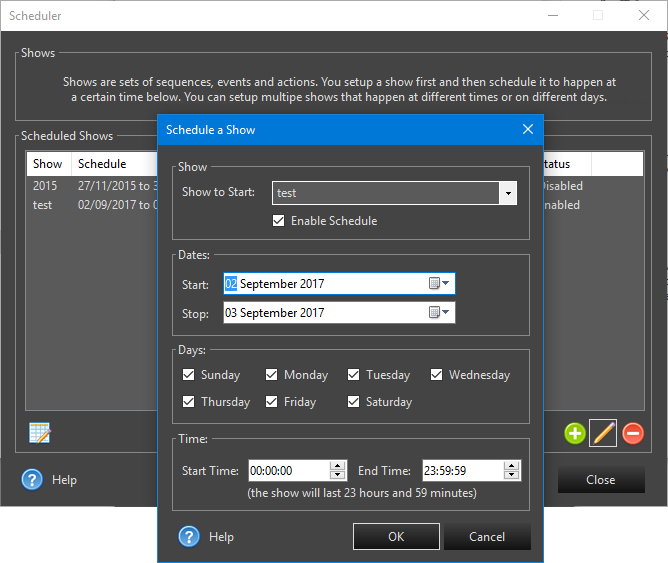
\includegraphics[width=0.8\columnwidth]{Figs/vixen_scheduler.png}
  \caption{\footnotesize Scheduler setup dialog}
  \label{fig:guide_scheduler}
\end{figure}

\section{VixenConsole CUI application}

To use the playback engine from command line, the CUI application \texttt{VixenConsole} is available. It is also optimised for Linux-based systems and mono runtime.

\newpage

\renewcommand{\baselinestretch}{1}
\begin{lstlisting}[language=]
Usage:  VixenConsole.exe [options] [commands...]

Options:
    -p itvl			| Start profiler with interval of itvl milliseconds
    -u playback			| Unlimit the update rate of playback frames
    -u controller		| Unlimit the update rate of controllers

Available commands:
    controller list		| List available controller modules
    controller config		| List current controller configurations
    tidy			| Remove unused sections from configuration files
    start file1 file2...	| Start playback with sequence file1 file2...

Supported sequence file formats:
    *_Network.xml		| Network configuration file from a raw sequence
    *.avi, *.mp4, ...		| Video sequence file

Configuration files:
    The controller configurations are read from the `Vixen 3' directory under
    user home directory. The directory structure and file formats are compatible
    with the Vixen GUI application.

Examples:
    VixenConsole.exe controller config
    VixenConsole.exe start exported_Network.xml exported.mp4
\end{lstlisting}
\renewcommand{\baselinestretch}{\mystretch}
